\pdfminorversion=7
\documentclass[12pt]{article}
\usepackage[utf8]{inputenc}
\usepackage[a4paper,margin=1in]{geometry}
\usepackage{amsmath,amssymb}
\usepackage{enumitem}
\usepackage{parskip}
\usepackage{hyperref}
\usepackage{xcolor}
\usepackage{fancyhdr}
\usepackage{tikz}
\usepackage{graphicx}
\usepackage{eso-pic}
\usepackage{titlesec}
\usepackage{pdfpages}
\graphicspath{{../../Hacking Session 1/}}

\definecolor{kcpc-bg}{RGB}{250,250,250}
\definecolor{kcpc-text}{RGB}{20,20,20}
\definecolor{kcpc-muted}{RGB}{90,90,90}
\definecolor{kcpc-red}{RGB}{176,0,0}
\hypersetup{
    colorlinks=true,
    urlcolor=kcpc-red,
    pdftitle={KCPC Hacking Session 3 Problems},
    pdfauthor={King's Competitive Programming Club}
}

\newcommand{\kcpcwordmark}{\raisebox{-0.15\height}{
\includegraphics[height=0.55cm]{kcpc-logo.png}}}

\pagestyle{fancy}
\fancyhf{}
\lhead{\textcolor{kcpc-text}{\small\bfseries Problems}}
\rhead{\textcolor{kcpc-muted}{\small Hacking Session 3}}
\cfoot{\textcolor{kcpc-muted}{\small KCPC}}
\renewcommand{\headrulewidth}{0.4pt}
\renewcommand{\headrule}{\hbox
to\headwidth{\color{kcpc-red}\leaders\hrule height \headrulewidth\hfill}}
\renewcommand{\footrulewidth}{0pt}
\setlength{\headheight}{28pt}

\AddToShipoutPictureBG*{%
    \begin{tikzpicture}[remember picture,overlay]
        \node[opacity=0.035, at=(current page.center)]
        {
\includegraphics[width=0.38\paperwidth]{kcpc-logo.png}};
    \end{tikzpicture}%
}

\titleformat{\section}{\large\bfseries\color{kcpc-red}}{\thesection}{1em}{}

\setlist[itemize]{noitemsep, topsep=4pt}
\setlist[enumerate]{topsep=4pt}

\title{KCPC Hacking Session 3 Problems\\NWERC 2025 and 2020}
\author{}
\date{}

\begin{document}
\maketitle
\thispagestyle{fancy}

\section*{Introduction}
\noindent
\textbf{Contest:} Northwestern Europe Regional Contest 2025 and 2020\\
\textbf{Problems:} 9, ordered from easiest to hardest

\begin{enumerate}
    \urlstyle{same}
    \renewcommand{\UrlFont}{\small}
    \item NWERC 2025 Fair Share: \url{https://codeforces.com/gym/106353/problem/F}
    \item NWERC 2025 Last Christmas: \url{https://codeforces.com/gym/106353/problem/L}
    \item NWERC 2025 Dreamcatcher: \url{https://codeforces.com/gym/106353/problem/D}
    \item NWERC 2025 KIT Finding: \url{https://codeforces.com/gym/106353/problem/K}
    \item NWERC 2025 Juggling Keys: \url{https://codeforces.com/gym/106353/problem/J}
    \item NWERC 2020 Dragon Balls: \url{https://codeforces.com/gym/103049/problem/D}
    \item NWERC 2025 Erratic Lights: \url{https://codeforces.com/gym/106353/problem/E}
    \item NWERC 2025 Arcade Crane: \url{https://codeforces.com/gym/106353/problem/A}
    \item NWERC 2020 Flight Collision: \url{https://codeforces.com/gym/103049/problem/F}
\end{enumerate}

{\small
Statements from the official \href{https://2025.nwerc.eu/problem-set.pdf}{NWERC 2025 booklet}
(\textcopyright\ 2025 by the NWERC 2025 jury, \href{https://creativecommons.org/licenses/by-sa/4.0/}{CC BY-SA 4.0})
and the \href{https://2020.nwerc.eu/files/nwerc2020problems.pdf}{NWERC 2020 booklet}.\par
}

\clearpage
% NWERC Statements.pdf contains these official PDF pages in ranked order.
% 2025 pp. 13-14, 25-26, 9-10, 23-24, 21-22; 2020 pp. 9-10;
% 2025 pp. 11-12, 3-4; 2020 pp. 13-14 (counting each booklet's cover).
% Compensate for the sub-point rounding of pdfTeX's full-page placement.
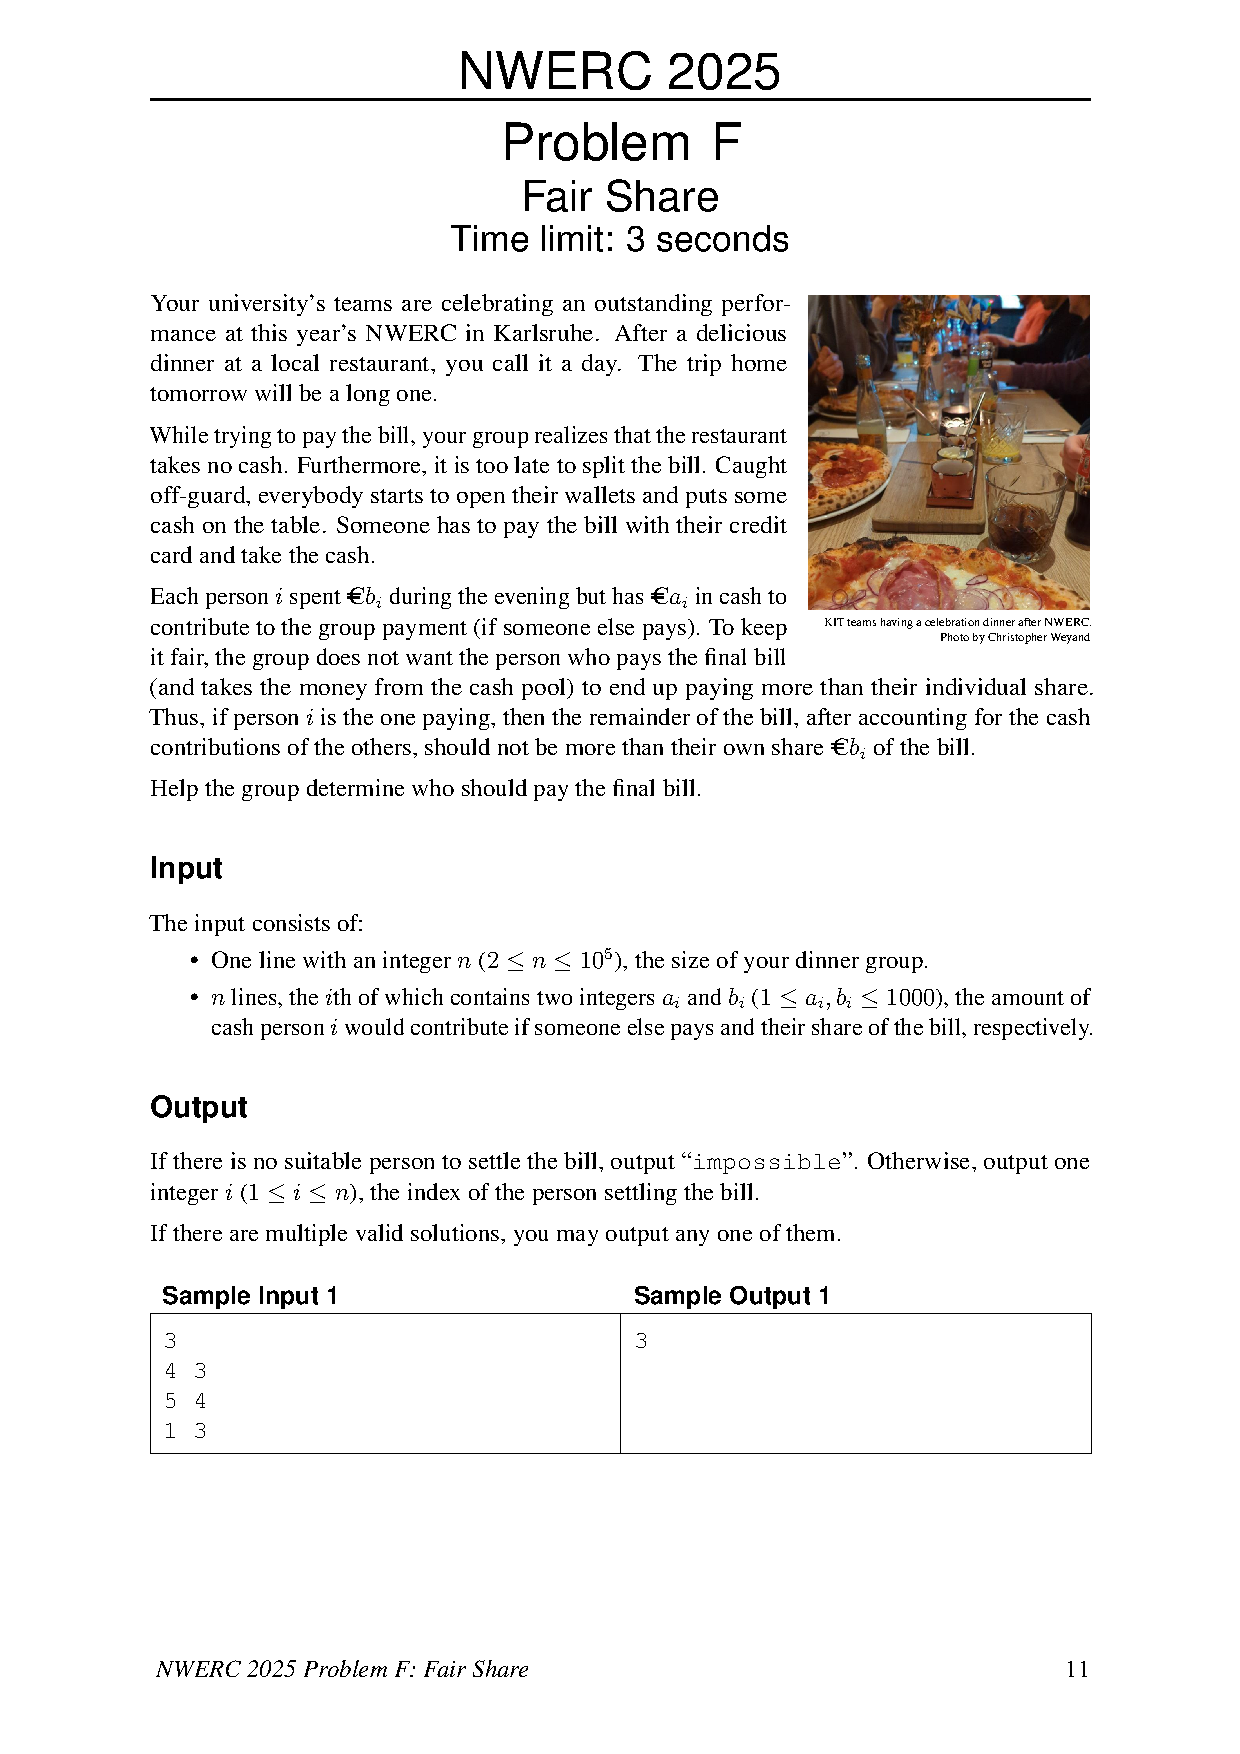
\includepdf[pages=-,noautoscale,offset=-0.001bp -0.001bp]{NWERC Statements.pdf}
\end{document}
